\documentclass[a4paper,12pt]{article}
\usepackage{geometry}
 \geometry{
 a4paper,
 total={170mm,257mm},
 left=20mm,
 top=20mm,
 }
\usepackage{adjustbox}
\usepackage[polish]{babel}
\usepackage{polski}
\usepackage{multirow}
\usepackage{makecell}
\usepackage{boldline}
\usepackage[T1]{fontenc} 
\usepackage{listings}
\usepackage{color}
\usepackage{biblatex}
\usepackage{csquotes}
\usepackage{indentfirst}
\addbibresource{docker.bib}

\lstset{literate={ą}{{\k{a}}}1 {ł}{{\l{}}}1 {ń}{{\'n}}1 {ę}{{\k{e}}}1 {ś}{{\'s}}1 {ż}{{\.z}}1 {ó}{{\'o}}1 {ź}{{\'z}}1 {Ą}{{\k{A}}}1 {Ł}{{\L{}}}1 {Ń}{{\'N}}1 {Ę}{{\k{E}}}1 {Ś}{{\'S}}1 {Ż}{{\.Z}}1 {Ó}{{\'O}}1 {Ź}{{\'Z}}1 {Ć}{{\'C}}1 {ć}{{\'c}}1 }

\title{Sprawozdanie z Zadania: Przygotowanie kontenera Docker z aplikacją webową}
\author{Jakub Kraus}
\date{24.01.2024}
\renewcommand\theadalign{tl}
\begin{document}
\renewcommand{\arraystretch}{2}
\begin{table}[ht]
    \centering
    \begin{adjustbox}{width=1\textwidth,center=\textwidth}
        \begin{tabular}{V{4}lV{4}c|c|c|c|c|c V{4}}
            \hlineB{4}
            \multicolumn{2}{V{4}lV{4}}{}                                         & \multicolumn{5}{lV{4}}{\textbf{Wydział Nauk Ścisłych i Technicznych}}                                                                                                                                   \\
            \cline{3-7}
            \multicolumn{2}{V{4}cV{4}}{\textbf{Uniwersytet Śląski w Katowicach}} & \multicolumn{5}{lV{4}}{\textbf{Instytut Fizyki}}                                                                                                                                                        \\
            \cline{3-7}
            \multicolumn{2}{V{4}lV{4}}{}                                         & Rok                                                                   & \textbf{III}                                          & Semestr                            & \multicolumn{2}{cV{4}}{\textbf{V}} \\
            \hlineB{4}
            Kierunek                                                             & \multicolumn{6}{cV{4}}{Informatyka stosowana}                                                                                                                                                           \\
            \hline
            Przedmiot                                                            & \multicolumn{6}{cV{4}}{\textbf{SiNWO - laboratorium}}                                                                                                                                                   \\
            \hlineB{4}
            Prowadzący                                                           & \multicolumn{6}{cV{4}}{dr Wojciech Gurdziel}                                                                                                                                                            \\
            \hline
            Tytuł ćwiczenia                                                      & \multicolumn{4}{c|}{\textbf{Wprowadzenie do konteneryzacji}}          &
            \multirow{2}{*}{Nr ćwiczenia}                                        & \multirow{2}{*}{\textbf{V}}                                                                                                                                                                             \\
            \cline{1-5}
            \thead{Sprawozdanie wykonał:                                                                                                                                                                                                                                                   \\ (Imię i Nazwisko)} &
            \multicolumn{4}{c|}{\textbf{Jakub Kraus}}                            &                                                                       &                                                                                                                                 \\
            \hlineB{3}
            Data wykonania ćwiczenia                                             & \textbf{24.01.2024}                                                   & \multicolumn{2}{V{4}lV{4}}{Data oddania sprawozdania} & \multicolumn{3}{cV{4}}{29.01.2024}                                      \\
            \hlineB{4}
        \end{tabular}
    \end{adjustbox}
\end{table}

\newpage

\tableofcontents

\newpage

\section{Cel ćwiczenia}
Celem ćwiczenia jest zapoznanie się z podstawowymi pojęciami związanymi z konteneryzacją oraz zbudowanie własnego obrazu Docker z aplikacją webową.

\section{Przebieg ćwiczenia}
Do wykonania ćwiczenia użyłem systemu \textbf{openSUSE Tumbleweed}\cite{noauthor_opensuse_nodate}, \textbf{Flask}\cite{noauthor_flask_nodate} do utworzenia aplikacji webowej przy użyciu Python'a oraz \textbf{Podman}\cite{noauthor_podman_nodate} jako zamiennik 1:1 dla dockera i można go zaliasować do
\begin{lstlisting}
    alias docker='podman'
\end{lstlisting}
Wybrałem go ponieważ jest otwartoźródłowy. Wszystkie polecenia wykonywałem w terminalu.

\subsection{Aplikacja Flask}

\subsubsection{app.py}

\begin{lstlisting}[breaklines=true, basicstyle=\small, numbers=left, language=Python]
from flask import Flask
from datetime import datetime

app = Flask(__name__)

@app.route('/')
def display_info():
    name = "Jakub Kraus"
    index_number = "344120"
    current_datetime = datetime.now().strftime("%Y-%m-%d %H:%M:%S")

    return f"{name}\n{index_number}\n{current_datetime}"

if __name__ == '__main__':
    app.run(debug=True, host='0.0.0.0', port=7777)

\end{lstlisting}
\subsubsection{requirements.txt}
\begin{lstlisting}[breaklines=true, basicstyle=\small, numbers=left]
    flask==3.0.0
    gunicorn==20.1.0
\end{lstlisting}
\begin{figure}

\end{figure}
\newpage

\subsection{Konteneryzacja\cite{noauthor_docker_2024}}
\subsubsection{Dockerfile}

\begin{lstlisting}[breaklines=true, basicstyle=\small, numbers=left]
    # Używamy obrazu Pythona w wersji 3.10, który jest lekki (slim).
    FROM python:3.10-slim
    
    # Otwarcie i przypisanie portu 7777, aby można było korzystać z aplikacji na tym porcie.
    EXPOSE 7777
    
    # Ustawiamy zmienną środowiskową, aby zapobiec tworzeniu plików pycache.
    ENV PYTHONDONTWRITEBYTECODE=1
    
    # Ustawiamy zmienną środowiskową, aby uniknąć buforowania w Pythonie.
    ENV PYTHONUNBUFFERED=1
    
    # Kopiujemy plik requirements.txt do obecnego katalogu.
    COPY requirements.txt .
    
    # Instalujemy zależności wymienione w pliku requirements.txt.
    RUN python -m pip install -r requirements.txt
    
    # Ustawiamy katalog roboczy na /app.
    WORKDIR /app
    
    # Kopiujemy wszystkie pliki z obecnego katalogu do katalogu /app w kontenerze.
    COPY . /app
    
    # Dodajemy użytkownika o identyfikatorze 5678, bez hasła, bez interaktywnego prompta.
    # Następnie zmieniamy właściciela katalogu /app na użytkownika appuser.
    RUN adduser -u 5678 --disabled-password --gecos "" appuser && chown -R appuser /app
    
    # Ustawiamy użytkownika appuser jako użytkownika, który będzie używany do uruchamiania kontenera.
    USER appuser
    
    # Komenda, która zostanie wykonana, gdy kontener zostanie uruchomiony.
    # Uruchamiamy Gunicorn (web server dla Pythona) naszej aplikacji na porcie 7777.
    CMD ["gunicorn", "--bind", "0.0.0.0:7777", "app:app"]
\end{lstlisting}


\newpage

\subsection{Budowa obrazu}
Aby zbudować obraz, należy wykonać polecenie:
\begin{lstlisting}[breaklines=true, basicstyle=\small, numbers=left]
    docker build -t sinwo:latest .
\end{lstlisting}

\begin{figure}[ht]
    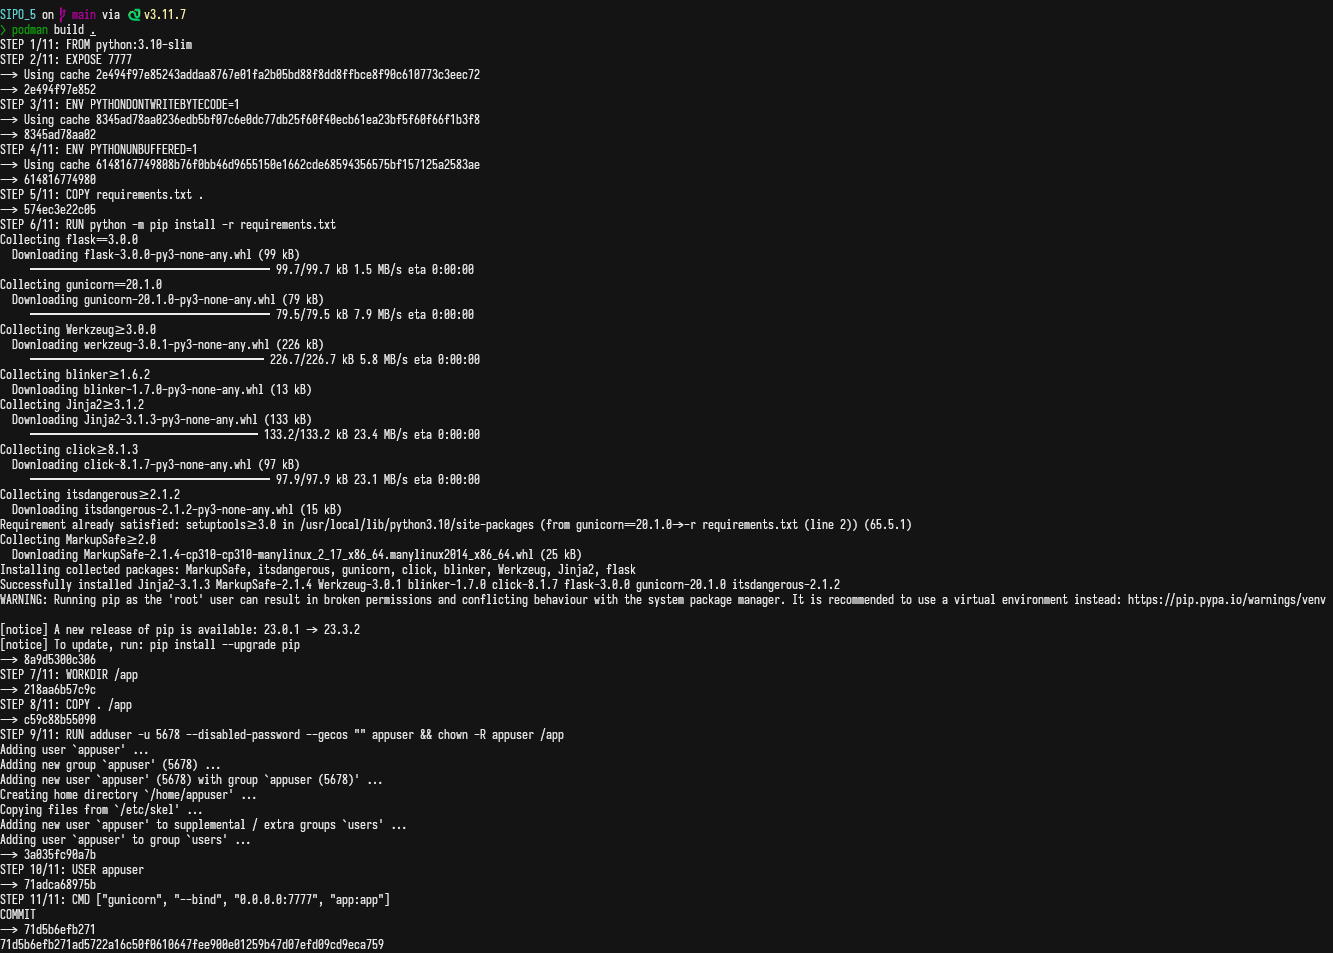
\includegraphics[width=1\textwidth]{images/docker_build.png}
    \caption{Wynik wykonania polecenia docker build}
\end{figure}
\subsection{Uruchomienie kontenera}
Aby uruchomić kontener, należy wykonać polecenie:
\begin{lstlisting}[breaklines=true, basicstyle=\small, numbers=left]
    docker run -d -p 8050:7777 sinwo:latest
\end{lstlisting}
\begin{figure}
    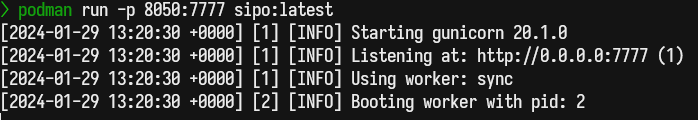
\includegraphics[width=1\textwidth]{images/docker_run.png}
    \caption{Wynik wykonania polecenia docker run}
\end{figure}
\newpage
\subsection{Umieszczenie obrazu w repozytorium}
Aby umieścić obraz w repozytorium, należy wykonać polecenia:

\begin{lstlisting}[breaklines=true, basicstyle=\small, numbers=left]
    docker tag sinwo:latest nazwa_użytkownika_repozytorium/sinwo:latest
    docker push nazwa_użytkownika_repozytorium/sinwo:latest
\end{lstlisting}

\begin{figure}[ht]
    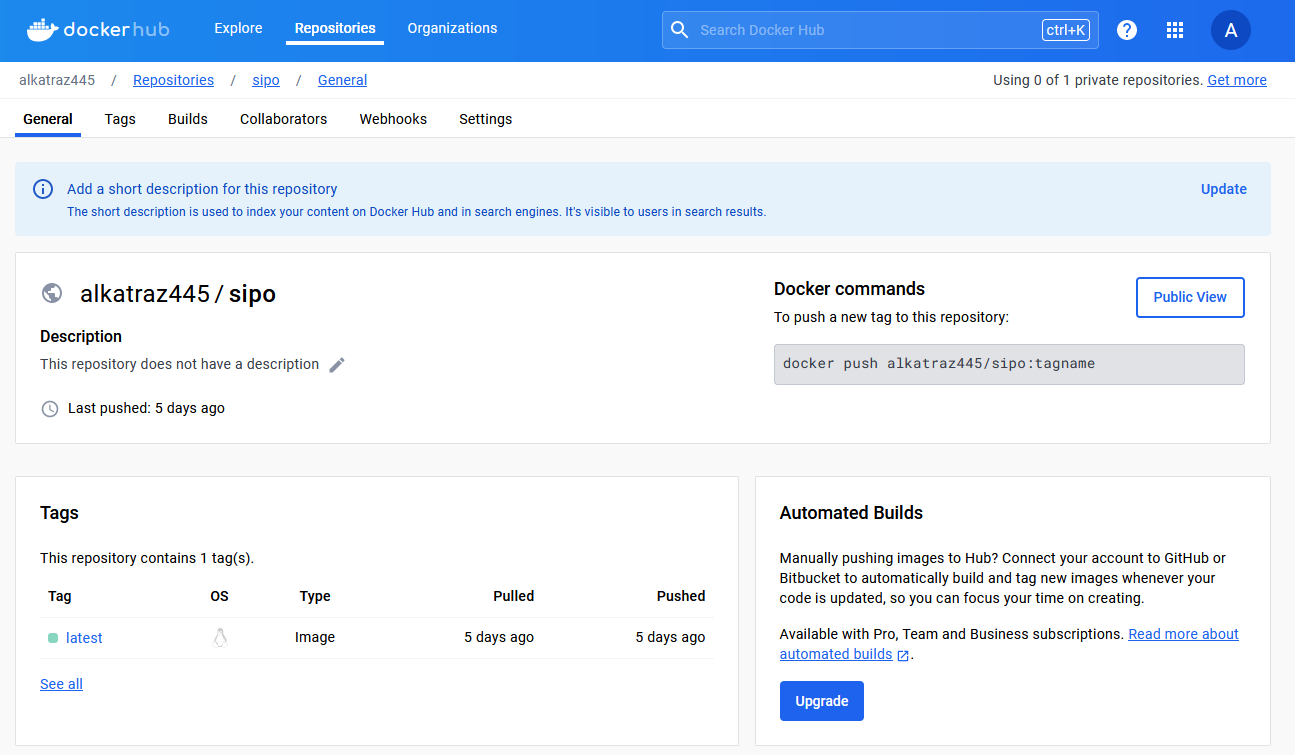
\includegraphics[width=1\textwidth]{images/docker_push.png}
    \caption{Docker Hub z obrazem\cite{kraus_docker_nodate}}
\end{figure}

\begin{figure}
    
\includegraphics[width=1\textwidth]{images/website.png}
    \caption{Strona internetowa}
\end{figure}

\newpage


\section{Wnioski}
Konteneryzacja pozwala na łatwe i szybkie uruchamianie aplikacji na różnych systemach operacyjnych. Dzięki temu, że kontenery są odizolowane od siebie, można uruchomić wiele kontenerów z różnymi aplikacjami na jednym systemie.

Tworzenie obrazów jest bardzo proste dzięki dockerfile, a dzięki temu, że można je umieszczać w repozytoriach, można łatwo udostępniać swoje aplikacje innym użytkownikom.

Cały proces używania kontenerów jest przystępny i łatwy do zrozumienia, co spowodowało gwałtowną adaptację w środowiskach produkcyjnych. Idea konteneryzacji również zapewnia, że nie pojawiają się problemy znane ze świata informatyki, takie jak ``U mnie działa''.

\printbibliography[heading=bibintoc]

Korzystałem również z pliku dostarczonego przez prowadzącego.

\end{document}